\section{單語言語音辨識系統架構}
在了解多語言辨識系統之前,必須先設計好一個足夠強大的單語言語音辨識系統,以深入且正確地探討多語言情景下的資訊。本論文所使用的單語言辨識系統架構如圖\ref{fig:chap3_framework}。
\begin{figure}[!h]
\centering
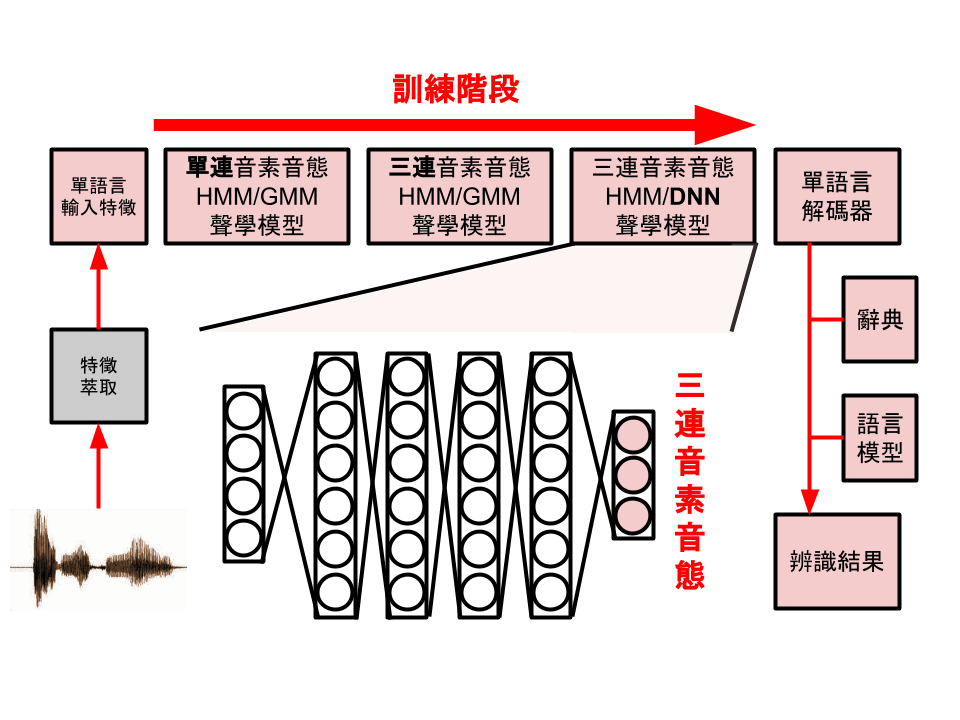
\includegraphics[scale=0.4]{images/chap3_framework.png}
\caption{單語言語音辨識統架構圖}
\label{fig:chap3_framework}
\end{figure}

本論文使用GP中的四個語言(西班牙語SP,捷克語CZ,法語FR,德語GE)做為實驗語料,因此會訓練出如圖\ref{fig:chap3_monolingual},四個互相獨立的單語言辨識系統,各自在自己的語言上辨識並回報結果。

四個語言分別有自己的訓練集(Training set)、發展集(Development set)以及測試集(Test set),由GP官方以8:1:1的比例設計,詳細數據請參考附錄。

\begin{figure}[!h]
\centering
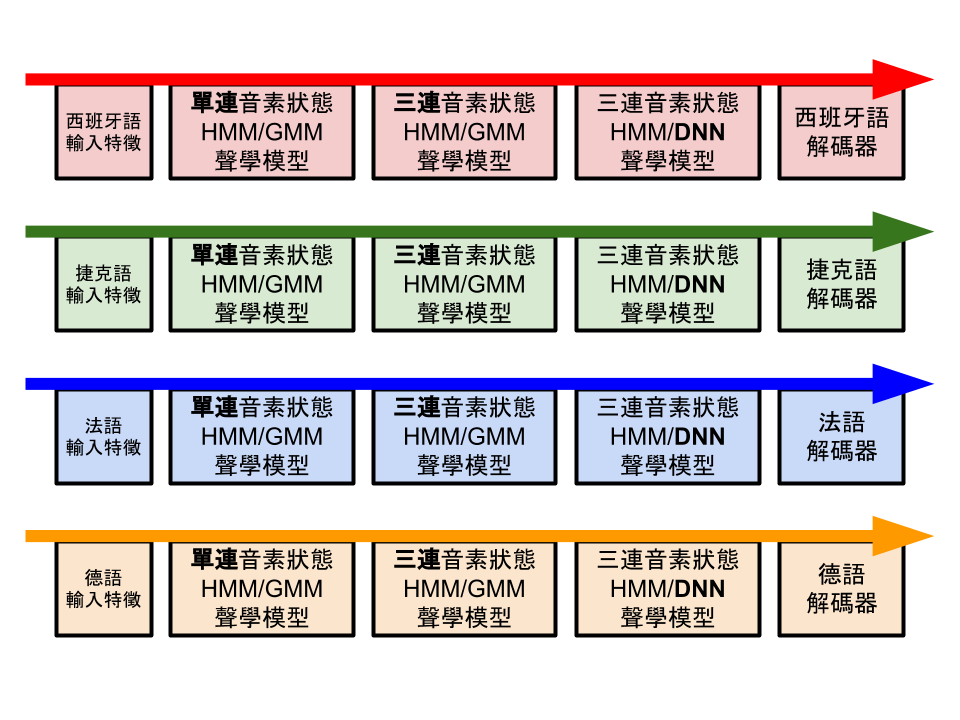
\includegraphics[scale=0.4]{images/chap3_monolingual.png}
\caption{西班牙語、捷克語、法語、德語的單語音辨識系統}
\label{fig:chap3_monolingual}
\end{figure}
\subsection{特徵萃取(Feature Extraction)}
給定麥克風收入的語音電訊號,特徵萃取旨在將此時頻訊號,轉換成更富含語言意義且較低雜訊的特徵向量,做為下一階段聲學模型的輸入。

特徵萃取階段,會從聲音訊號中取出寬度25毫秒的音框(Frame)。針對一句話連續取樣音框時,音框中心點間隔10毫秒,因此必然有重疊部分,以降低邊界雜訊。每個音框內計算訊號的梅爾頻率濾波組(Mel-frequency Filterbanks, FBANK),取其不包含能量(Energy)的23維頻率強度。一個音框為模型的一筆訓練實例(Training Instance)。

這23維特徵,會經過一階差分以及二階差分,計算出總計69維的輸入特徵。接著經過語者譜頻平均正規化(Speaker-wise Ceptral Mean Normalization, CMN),分別調整各維度的值,使得同樣語者分佈在不同句子的所有訓練實例中,同維度的平均值皆為0。正規化能夠一定程度地降噪,同時能有效降低語者之間的差異性,使得不同語者的聲音都能轉換在共同的輸入空間上設計系統。

然語音乃高度結構化的訊號,訓練深層類神經網路的時候,還會把單一音框和前後文(Context)音框同時黏合起來。以前四後四為例,對每一個訓練實例,把前後各四個音框的向量與之結合,形成總共$69 \times (4 + 1 + 4) = 621$維的輸入向量。前後文相依(Context-dependent, CD)提供更強大的預測能力,對於深層類神經網路的模型訓練複雜度幾乎沒有影響,卻對高斯混合模型造成強大的訓練時間懲罰。

\subsection{聲學模型(Acoustic Modeling)}
給定萃取後的特徵向量序列,聲學模型旨在將此序列轉換成對應的發音單位序列,經過辭典(Lexicon)轉換成有文字意義的詞彙序列,做為下一個階段語言模型的輸入。

聲學模型乃利用數學模型得到以下的機率:
\begin{equation}\label{eq:am}
p( \bold{s} | \bold{x}_1 , \bold{x}_2 , ... , \bold{x}_T ) = \frac{ p( \bold{x}_1 , ... , \bold{x}_T | \bold{s} )p( \bold{s} )}{ p( \bold{x}_1 , \bold{x}_2 , ... , \bold{x}_T ) }
\end{equation}

其中$\bold{s} = \{s_1 , s_2 , ... , s_T \}$是發音單位的序列,$\bold{x}_t$為輸入的第$t$個音框特徵向量,一句話總計有$T$個音框。

公式\ref{eq:am}根據貝式定理(Bayes Theorem),針對整句話的發音單位建模。因此,整個模型拆解成兩個部分,一個為發音單位之間變化的轉移模型(Transition Model)如公式\ref{eq:am_trans}。
\begin{equation}\label{eq:am_trans}
p( \bold{s}) = p(s_1)\prod_{i=2}^{T} { p( s_i | s_{i-1} ) } 
\end{equation}

以及單音框內發音單位與特徵向量的分布模型(Emission Model),如公式\ref{eq:am_emit}。

\begin{equation}\label{eq:am_emit}
p( \bold{x}_1 , \bold{x}_2 , ... , \bold{x}_T | \bold{s} ) = \prod_{i = 1}^{T} p( \bold{x}_i | s_i )
\end{equation}

使用聲學模型時,旨在找到最可能的發音單位序列能夠最大化這個機率:
\begin{equation}\label{eq:am_argmax}
 \bold{s}^* =  \arg\max_{\bold{s} } \frac{ p( \bold{x}_1 , ... , \bold{x}_T | \bold{s} ) p( \bold{s} ) } { p( \bold{x}_1 , \bold{x}_2 , ... , \bold{x}_T ) } = \arg\max_{\bold{s} }  p( \bold{x}_1 , ... , \bold{x}_T  | \bold{s} ) p( \bold{s} ) 
\end{equation}

其中轉移模型利用馬克夫鏈(Markov Chain)的概念,將每一個發音單位的分布機率限定在只根據前一個發音單位。分布模型則把每一個音框的相依性拆開,使得整個序列的分布機率僅為個別音框的分布機率乘積。

在替分布模型建模的時候,最原始的作法是使用高斯混和模型(Gaussian Mixture Model, GMM),替每一個發音單位,用一把不同權重的高斯分布加權總合計算出機率。因為以高斯函數計算機率的運算複雜度受維度大小影響甚大,為了保持可接受的運算時間,通常僅根據於69維的FBANK特徵建模。

進階的分布模型建模時,可以將原本替個別音框分布機率的公式\ref{eq:am_emit},再度以貝式定理拆開,如下:
\begin{equation}\label{eq:am_emit_framewise}
p( \bold{x}_i | s_i ) = \frac{ p( s_i | \bold{x}_i) p( \bold{x}_i ) } { p ( s_i )}
\end{equation}

其中$p(\bold{x}_i )$會在使用聲學模型時,如同公式\ref{eq:am_argmax}時一樣捨棄掉。$p( s_i )$為該發音單位的事前機率,可以藉由統計所有音框的發音單位來獲得。$p( s_i | \bold{x}_i )$為一個分類器問題,給定輸入特徵向量$\bold{x}_i$,分類為發音單位$s_i$的機率,可以使用深層類神經網路來建模,以及$621$維的高維度輸入特徵,以達到更好的預測準確率。

在替轉移模型建模時,必須先決定好建模所使用的發音單位。語言學家定義音素(Phone)為人耳可鑑別的最小發音單位,然對於機器而言,音素的層級太過粗糙,無法囊括聲音訊號的變化。最原始的做法是使用隱藏式馬可夫模型(Hidden Markon Model, HMM)作為轉移模型,將每一個音素拆解成三種發音狀態,稱為單連音素音態(Monophone state)。

然以單連音素音態作為發音單位仍然不夠細緻,因為音素在不同的前後文(Context)中,依然有不同的特徵表現。因此,考慮三個連續音素的組合變化,把一組三連音態用三種發音狀態拆解,稱為三連音素音態(Triphone state)。因為音素約莫40個,三連音態的組合便有$40^3 \times 3= 192000$種三連音素音態。這個輸出維度太過龐大,某些組合的資料量太小,因此有些相近的三連音素音態會合併起來視為同一種發音單位。

整個聲學模型的訓練過程,就是一種由淺入深的過程。萃取好特徵向量之後,一步一步將發音單位磨得越來越細緻。回顧圖\ref{fig:chap3_framework},一開始建立HMM與GMM的單連音素音態模型,然後拆解成三連音素音態的模型,最後把高斯混合模型切換成深層類神經網路,重新建模。

有了聲學模型,利用公式\ref{eq:am_argmax}能夠找出最好的發音單位序列,搭配辭典,可以將發音單位序列組合成字或詞的序列。實務上,聲學模型會保留機率夠高的多組序列輸出,以免因為模型誤差把可能的正確序列提早屏除掉了。

\subsection{語言模型(Language Modeling)}

給定聲學模型篩選出的字詞序列,語言模型可以根據字詞之間的意義相關性與文法合理,給予語言知識上的評分。

給定詞序列,語言模型在於估計以下機率:
\begin{equation}
p( w_1 , w_2 , w_3 , ... , w_L )
\end{equation}
其中L為該序列對應的詞的數量,$w_i$為序列中的詞。

一般而言,常用多連文法(N-gram)來建模:
\begin{equation}
p( w_1 , w_2 , w_3 , ... , w_L ) = \prod_{i = 1}^L p( w_i | w_{i-1} , w_{i-2} , ... , w_{i-N+1} )
\end{equation}

N的決定來自於系統規模的考量。產品設計上可能會到4,5甚至6,研究上取N=3,三連文法即足夠。

由於語言模型是跳脫於語音文件外的,因此通常可以採用額外的巨量數據來補足,形成背景模型(Background Model)。如果語音辨識時能夠知道文字的特定領域,例如是否屬於報章雜誌?還是科技期刊?或是網路討論?情感抒發?不一樣的文字內容,亦可能需要不同的語言模型來建模。這些針對的領域模型(In-domain Model),還可以與背景模型加權平均,形成內插模型(Interpolation Model)。內插模型能夠提供背景模型的強大力量,又能針對領域與特定知識提供分數,往往擁有較好的表現。

\subsection{解碼器(Decoder)}
有了聲學模型、語言模型,解碼器旨在把所有的模型統合起來,形成一個由聲音訊號到文字序列的辨識系統。

理論上,聲學模型、辭典、語言模型是三個輸入與輸出剛好匹配的系統,能夠一直線到底完成系統。實務上,為了整體系統設計更為穩健,避免前端系統的錯誤提早刪去正確序列,解碼器的演算法設計除了著重時間、空間複雜度之外,還須考量模型的彈性。這包含:

\begin{itemize}
\itemsep -2pt %reduce space between items
  \item 語音辨識是在整個輸入向量空間中,樹狀搜尋分數最高的一條路線。然樹狀分支會隨著解碼序列增長而變得龐大,因此必須進行光束刪減(Beam Pruning),在某時刻只保留部份最具可能性的序列,傳遞至下一階段。這個保留的比例是系統設計的一個彈性參數,保留越少越需要的解碼時間越短,但卻可能提早把正確序列捨棄掉。

 \item 語音辨識中,聲學模型與語言模型各自佔有不同的地位。前者試著保留聲音以及發音單位的關聯性,後者則估計不同字詞間相連的合理性。這兩者的權重比例是解碼器設計的一個彈性。前者的比例越高,表示系統越重視聲學模型所訓練出來的聲音,但卻可能讓出來的文字序列意義不彰。

 \item 語音辨識系統由許多不同的子系統組合而成,各自蓬勃發展,系統必須要支援各個子系統的熱插拔(Plug and Play, PnP),能夠彈性地切換不同的聲學模型、語言模型以及辭典。
\end{itemize}

現在的語音辨識解碼器演算法,通常根據於加權有限狀態傳感器(Weighted Finite State Transducer, WFST),將不同的模型轉換成WFST的格式儲存在電腦或是雲端的記憶體裡。如:



\begin{table}[htbp]
%\resizebox{\columnwidth}{!}{
\centering
\begin{tabular}{|cccl|}
\hline
 代號 & 輸入 & 輸出 & 備註 \\
\hline
 U    & 三連音素音態 & 三連音素音態 & 權重為聲學模型分佈機率 \\
\hline
 H    & 三連音素音態 & 三連音素音態 & 權重為聲學模型轉移機率 \\
\hline 
 C    & 三連音素音態 & 音素 & 無權重  \\
\hline
 L    & 音素 & 詞 & 無權重,由辭典產生,將可能的音素對應回詞 \\
\hline
 G    & 詞 & 詞 & 權重為語言模型詞序機率   \\
\hline

\end{tabular}
\caption{解碼器相關WFST的輸入輸出與權重意義}
\label{table:chap3_wfst}
\end{table}

語音辨識模型中,聲學模型、辭典以及語言模型能夠分別轉換化成對應的H、C、L、G,並且組合(Composition)成一個統一的WFST,合稱HCLG,是辨識系統的核心本體。每當一段聲音訊號進入,系統會先進行特徵萃取,將萃取好的特徵向量序列,輸入訓練好的深層類神經模型,產生出一個句子的WFST,為表\ref{table:chap3_wfst}中的U。

U會與記憶體裡的HCLG再度組合(Composition),形成U-HCLG。組合過程中的U-HCLG佔據非常大的記憶體,因此在組合過程中便會進行光束刪減(Beam Pruning)。組合完畢的U-HCLG再經由WFST的最短路徑(Shortest-path)演算法,找到分數最高的一條路徑,將路徑上的詞序全部輸出,即為辨識結果。辨識結果與語料庫提供的正確詞序比較,得到詞誤率(Word Error Rate, WER),作為評估的考量。詞誤率是評估語音辨識最重要的參數之一,越低代表著辨識系統錯誤的詞越少。

研究上,聲學模型的訓練過程,以及解碼器的諸多彈性參數,都必須根據情景調整,沒有一個通用的最佳解。學術上的慣例會以語料庫中的訓練集作為訓練模型的資料,而以發展集作為調整解碼器的參數,如光束大小、語言模型的權重等等。
\section{深層類神經網路基礎實驗設計}
本論文評估單語言語音辨識系統的基礎實驗設計,旨在探討語言模型、丟棄演算法、深層類神經網路的參數設定,作為之後多語言語音辨識系統的基準實驗。
\subsection{語言模型}
評估語言模型的方式有兩種方式,一種為混淆度(Perplexity),用以衡量語言模型於給定測試語料的分數,公式如下:
\begin{equation}
PPL(w_1 , w_2 , w_3 , ... , w_L ) =  p(w_1 , w_2 , w_3 , ... , w_L ) ^{-\frac{1}{L}}
\end{equation}
混淆度越大,表示語言模型在預測該文字測試語料的信心指數越低。

% TODO REF SRILM
評估單語言語音辨識系統之前,本論文使用三種不同的語言模型,分別針對GP的純文字測試語料計算混淆度。三種模型分別為:

\begin{table}[htbp]
%\resizebox{\columnwidth}{!}{
\centering
\begin{tabular}{|c>{\columncolor{red!20}}c>{\columncolor{green!20}}c>{\columncolor{blue!20}}c>{\columncolor{yellow!20}}cc|}
\hline
 模型名稱 & 西班牙語 & 捷克語 & 法語  & 德語 & 備註 \\
\hline
 背景模型 & 1.40M    &  1.05G & 85.3M & 66.9M & GP官方提供的語言模型 \\
\hline
 領域模型 & 2.74M    &  3.57M & 4.08M & 3.73M & 使用GP訓練語料文字訓練而成 \\
\hline
 內插模型 & 3.15M    &  468M  & 87.1M & 67.2M & 等比例內插背景模型以及領域模型 \\
\hline
\end{tabular}
\caption{四個語言分別三種不同語言模型的模型大小。官方提供的西班牙語語言模型規模小,嚴格來說不像是背景模型。捷克語的內插模型過大,因此有使用辭典刪減不在訓練集內的詞的參數。}
\label{table:chap3_lm_stat}
\end{table}


三個模型除了混淆度之外,亦會與深層類神經網路的聲學模型結合,計算詞誤率,結果如表\ref{table:chap3_lm}。



\begin{table}[htbp]
%\resizebox{\columnwidth}{!}{
\centering
\begin{tabular}{|cc>{\columncolor{red!20}}c>{\columncolor{green!20}}c>{\columncolor{blue!20}}c>{\columncolor{yellow!20}}c|}
\hline
 語言模型 & 評估指數 & 西班牙語 & 捷克語 & 法語 & 德語 \\
\hline
 \multirow{2}{*}{背景模型}&      PPL & \underline{161} & 1421 & 357 & 680 \\
        &      WER & \underline{8.68\% } & \underline{18.13\% } & 20.87\% & 17.85\% \\
\hline
 \multirow{2}{*}{領域模型}&      PPL & 284 & \underline{1076} & \underline{275} & 934 \\
        &      WER & 23.76\% & 43.19\% & 22.86\% & 19.51\% \\
\hline
 \multirow{2}{*}{內插模型}&      PPL & 206 & 1317 & \underline{284} & \underline{641} \\
        &      WER & 10.34\%  & 20.12\%  & \underline{17.21\%} & \underline{15.28\%} \\
\hline
 官方數據 &      WER & 10\%  & 15.7\%  & 19.5\% & 14.2\% \\
\hline
\end{tabular}
\caption{四個語言的單語言辨識系統在不同語言模型下的詞誤率,包含語言模型在相應的測試集計算而得的混淆度。表中的詞誤率計算,都是使用4層寬度為2048神經元並使用S型函數作為活化函數的深層類神經網路聲學模型。}
\label{table:chap3_lm}
\end{table}

從表\ref{table:chap3_lm}可以看到混淆度與詞誤率有一定程度的正相關,混淆度越低通常意味著詞誤率越低。然在計算詞彙外(Out-of-Vocabulary, OOV)的詞時,混淆度會直接跳過不納入考量,而詞誤率則會直接反應在數據上。即便捷克語以及法語的領域模型混淆度都較低,該語言模型在詞誤率的表現卻很差,因為領域模型的訓練資料只有GP的訓練集的句子,資料相比背景模型而言少非常多。

內插模型擁有領域模型的豐富資訊,和領域模型的特定資訊,因此在法語跟德語上表現結果較好。西班牙語跟捷克語的訓練集較不匹配測試集,使用背景模型本身比較好,加入領域模型沒有提供更多資訊。

之後的實驗針對不同語言,解碼器所使用的語言模型,為本表格中測試詞誤率最低的相應語言模型。然而,這個行為違反了機器學習的驗證理論,理論上不應該從測試集的結果中進行挑選。但本研究核心內容著重在聲學模型的設計與實驗比較,為了建立較強力的基準實驗系統,特意揀選語言模型。之後實驗亦不再多做討論語言,僅在此呈現數據。


\subsection{丟棄演算法}
深層類神經網路深受過度貼合的影響,丟棄演算法是典型的控制適應來避免過度貼合。然丟棄演算法的隨機性會破壞訓練的穩定度,在過程中強制關閉神經元輸出,會丟棄神經網路學到的資訊。一般而言,語音訊號的丟棄比例設定在$0.05 - 0.1(5\% - 10\%)$之間。本實驗的丟棄比例為0.1,即10\%。

一般的類神經網路會使用S型函數作為活化函數。S型函數在接近0的位置變化量最大,因此能夠拉開神經元在接近閾值時的些微變化,讓神經網路對於細微的差異更為敏銳。
使用丟棄演算法的類神經網路,會因為丟棄的隨機性讓S型函數的反應呈現較多的雜訊,訓練上不穩定。因此,搭配丟棄演算法通常會使用線性整流子(ReLU)作為活化函數。


\begin{table}[htbp]
%\resizebox{\columnwidth}{!}{
\centering
\begin{tabular}{|c>{\columncolor{red!20}}c>{\columncolor{green!20}}c>{\columncolor{blue!20}}c>{\columncolor{yellow!20}}c|}
\hline
 方法    & 西班牙語 & 捷克語 & 法語 & 德語 \\
\hline
  S型函數(無丟棄)& 8.74\% & 18.16\% & 17.43\% & 15.85\% \\
\hline
  線性整流(丟棄10\%)& \underline{8.58\%} & \underline{17.61\%} & \underline{17.15\%} & \underline{15.40\%} \\
\hline
\end{tabular}
\caption{四個語言的單語言辨識系統詞誤率,比較聲學模型的類神經網路有無使用丟棄演算法。表中的類神經網路模型都是4層寬度2048神經元。}
\label{table:chap3_dropout}
\end{table}

結果如表\ref{table:chap3_dropout},丟棄演算法的結果顯然幫助了詞誤率的降低,對於所有語言都有一致的效果,已是使用深層類神經模型建立語音辨識系統的典型方法。

如未特別提示,往後的實驗皆使用線性整流子以及10\%的丟棄演算法。

\subsection{模型深度}

深層類神經網路的深度,指的是模型中疊起的隱藏層數量,是模型重要的參數設計。越深的模型,意味著更有能力一層一層剖析輸入向量的資訊,分門別類,越接近輸入端的隱藏層擁有類似特徵過濾(Feature Filtering)的降噪功能,能夠找到頻譜資訊(Spectral Information);越接近輸出端的隱藏層,則是擁有高階的分類資訊,能夠將過濾好的隱藏層正確分類成指定類別。然而,較深的類神經網路,意味著訓練時更高的困難度。因為使用一般的反向傳播與機率性梯度降低演算法優化模型時,容易發生梯度消失(Vanishing Gradients),使得前端的神經網路參數不容易被更新到。


\begin{table}[htbp]
%\resizebox{\columnwidth}{!}{
\centering
\begin{tabular}{|cc>{\columncolor{red!20}}c>{\columncolor{green!20}}c>{\columncolor{blue!20}}c>{\columncolor{yellow!20}}cc|}
\hline
 深度  & 寬度  & 西班牙語 & 捷克語 & 法語 & 德語 & 參數數量 \\
\hline
  4    & 2048   & 8.58\% & 17.61\% & 17.15\% & 15.40\% & 75.6M \\
\hline
  7    & 2048   & \underline{8.41\%} & \underline{17.03}\% & \underline{16.80\%} & \underline{14.50\%} & 126.4M \\
\hline
\end{tabular}
\caption{四個語言的單語言辨識系統詞誤率,比較不同深度的模型比較。表中所有的深層類神經網路模型都是線性整流子以及丟棄比例10\%的結果。}
\label{table:chap3_depth}
\end{table}

表\ref{table:chap3_depth}中,越深的類神經網路模型效果越好。但笨重的7層深層網路模型,無論是順向預測或是反向傳播的時間都高上許多,不適合進行即時(Real-time)語音辨識,也不適合放在隨身裝置上,也因此小型模型如4層的深層類神經網路,仍然有其參考價值在,因為他的模型大小為0.6倍,但結果差異只有1\%左右。
\subsection{基準實驗總結}
單語言語音辨識系統的基準實驗,除了比較語言模型外,改動了聲學模型中的深層類神經網路訓練架構及演算法。實驗設計上先以經典的S型函數著手,嘗試加上丟棄演算法、線性整流子作為控制調適,同時比較兩種不同深度的深層類神經網路結果與參數數量。

其中,語言模型只挑選最好的結果給之後的實驗使用;S型函數為經典深層類神經網路的結果,是之後比較多語言語音辨識系統的重要指標;不同深度的深層類神經網路,也是之後比較知識蒸餾中重要的參考數據,也是基準實驗中詞誤率最好的結果。

